\documentclass[a4paper]{article}

\usepackage[latin1]{inputenc} % LaTeX, comprends les accents !
\usepackage[T1]{fontenc}      % Police contenant les caractères français
\usepackage{geometry}         % Définir les marges
\usepackage[francais]{babel}  % Placez ici une liste de langues, la
\usepackage{graphicx}
\usepackage{placeins}
\usepackage{listings}

\title{NA62 RunControl FSM}           % Les paramètres du titre : titre, auteur, date
\author{Nicolas Lurkin,  Riccardo Fantechi,  Gianluca Lamanna,\\ Fernando Varela Rodriguez, Marco Sozzi}

\begin{document}

\maketitle                  % Faire un titre utilisant les données


\begin{figure}[hn]
	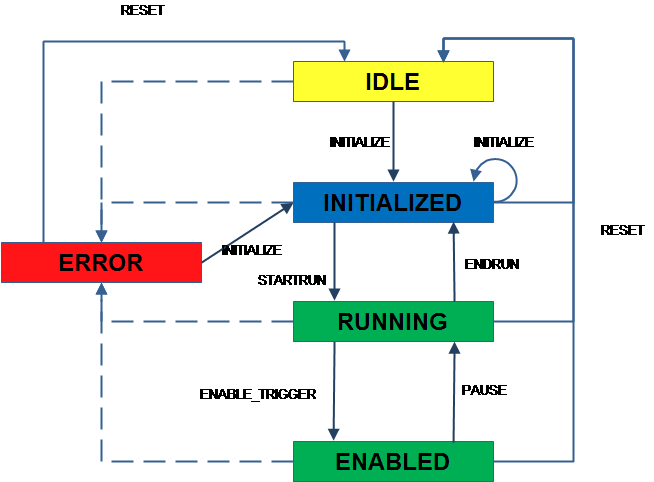
\includegraphics[width=\textwidth]{NA62FSM2.png}
	\caption{FSM diagram for logical detector}
\end{figure}

The FSM diagram above will be used for each logical detector (subdetectors and top node). This document will describe each state and the commands associated. Each command triggers actions both on the devices (boards and scripts) and in the FSM User interface, possibly requiring action from the shifter. It will be presented in the logical order of operating the detector.

%\section{NOT\_LOADED}
%This is the initial state right after starting the FSM.
%
%
%\paragraph{LOAD} This command will ask the configuration tool to connect to the database and allow the FSM to go to the IDLE state.

\section{IDLE} 
This is the initial state after starting the FSM and the devices. At this level, no action has been taken on the devices.

\paragraph{INITIALIZE} When asking for the INITIALIZE command, a popup will first appear, asking the shifter to choose the type of run. Depending on the type of run, different configuration files will be used. The correspondence between the configuration files and the type of run is stored in a database. The configuration tool will load the correct file path and each device will then apply it.

\section{INITIALIZED}
When the devices report that they applied the configuration file properly, the FSM moves to the INITIALIZED state. At this stage, the INITIALIZE command is still available to allow for the possibility of re-initializing the devices with another set of configuration files.

\paragraph{STARTRUN} A popup appears providing the following information about the run: 
\begin{itemize}
	\item Run type
	\item Run number
\end{itemize}
The shifter is asked to input the following ones: 
\begin{itemize}
	\item Type of beam
	\item Shifter(s) name(s)
	\item Start of run command
\end{itemize}
If the possibility of retrieving the type of beam automatically from the beam department is given, this will not more be asked to the shifter.
Once the validate button is clicked, an archive directory and a summary XML file are created. The name of the directory is "RunX", X being the run number. All the configuration files that were used are copied in this directory with the filename following this convention: "devicename\_timestamp\_originalfilename.ext". The XML file\footnote{An example XML file is given in annex of this document.} is already filled with the following values:
\begin{itemize}
	\item Run number
	\item Run type
	\item Run start time
	\item Start of run comment
	\item Shift crew
 	\item Beam type
	\item A list of the subsystems and for each the configuration filename and the timestamp at which it has been saved.
\end{itemize}
In addition to this, the \textit{page 1} message from SPS will be shown and logged in the XML file during the run.
All the devices except the L0TP are then asked to move to the RUNNING state. They will be ready to take data as soon as the trigger is received. 

\section{RUNNING}
In this state, all the devices are already in their RUNNING state but don't receive triggers: the L0TP is the only one that did not received this command yet. This state allows to pause a run.

\paragraph{ENABLE\_TRIGGER} This command will just send the startrun command to the L0TP that will dispatch the trigger.

\paragraph{ENDRUN} This command will trigger the end of the run. All the devices will receive this command and will possibly execute some end of run script (TEL62). A popup appears and ask the shifter to input a comment. The configuration files used for this run are again copied in the archive directory following the same convention as for the STARTRUN command and the following values are appended to the XML file:
\begin{itemize}
	\item Run end time
	\item End of run comment
	\item A list of the subsystems and for each the configuration filename and the timestamp at which it has been saved.
\end{itemize}

\section{ENABLED} All the devices are in their RUNNING state, the triggers are dispatched and the experiment is effectively taking data.

\paragraph{PAUSE} This command will pause the running by asking the L0TP to stop dispatching the trigger.

\section{ERROR} This state can be reached from any other state whenever a problem occurs in a device. The reasons can be multiple: configuration file not loaded properly, error in the program/configuration and the state of the device becomes unstable while running,...
When an error occurs, the PAUSE command is emitted and the shifter will then decide to try to recover from the error or stop the run.

\paragraph{RECOVER/INITIALIZE} This command is used to recover from an error but is effectively the same as the INITIALIZE command and therefore is named INITIALIZE in the FSM.

\paragraph{RESET} This command is available from every state and is used to return any device to its IDLE state.


\section{GLOBAL/LOCAL mode}
Switching between LOCAL and GLOBAL mode is slightly different from the other commands as GLOBAL/LOCAL is not a state in the FSM. We will use the partitioning tool provided by the framework. When the first user takes the ownership of the FSM, the appropriate command is sent to the LTUs to switch them all to GLOBAL. When a subdetector is released from the main FSM and the ownership is taken by a second user, the command is sent to the LTU to switch to local mode and a different configuration is loaded in the TEL62 board in order to send the data to a different PC. Switching between GLOBAL/LOCAL will only be possible when in IDLE or INITIALIZED state. No change is allowed in the RUNNING or ENABLED states.

\newpage

\section{Example XML File}
\lstinputlisting{RunSummary.xml}
\end{document}
